\documentclass[12pt,letterpaper, onecolumn]{exam}
\usepackage{amsmath}
\usepackage{pdfpages}
\usepackage{amssymb}
\usepackage{graphicx}
\usepackage{setspace}
\usepackage{nicefrac}
\usepackage{hyperref}
\setcounter{MaxMatrixCols}{20}
\usepackage[lmargin=71pt, tmargin=1.2in]{geometry}  %For centering solution box
\lhead{Principles of Navigation}
\rhead{Noah Miller}
\thispagestyle{empty}   %For removing header/footer from page 1

\begin{document}

\begingroup
\centering
\LARGE Principles of Navigation\\
\LARGE Homework 2 \\[0.5em]
\large \today\\[0.5em]
\large Noah Miller\par
\large 903949330\par
\large MECH 6970\par
\endgroup
\pointsdroppedatright   %Self-explanatory
\printanswers
\renewcommand{\solution}{\noindent\textbf{Answer:}\enspace}   %Replace "Ans:" with starting keyword in solution box



\begin{questions}
    \question{}
    \begin{parts}
        \part{}

        \part{}

        \part{}

        \part{}

    \end{parts}
    \clearpage
    \question{Consider the three-link, planar robot shown below for which four coordinate frames have been assigned. Frame $\{0\}$ is fixed, frame $\{1\}$ rotates with angle $\theta_1$ relative to Frame $\{0\}$, frame $\{2\}$ rotates with $\theta_2$ relative to frame $\{1\}$, and frame $\{3\}$ translates with distance $d_3$ relative to frame $\{2\}$.

        \begin{figure*}[!h]
            \centering
            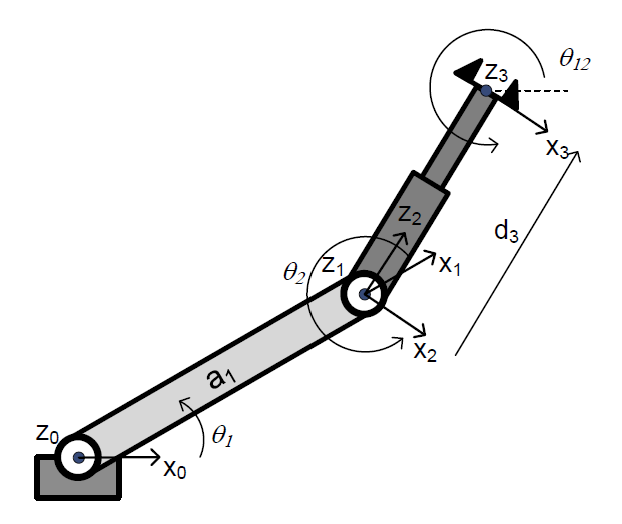
\includegraphics[width=0.5\linewidth]{Q2ps.png}
        \end{figure*}

        The rotation matrices and displacements between frames are shown below.
        \centering
        $\mathbf{C_1^0} =
            \begin{bmatrix}
                c_1 & -s_1 & 0 \\
                s_1 & c_1  & 0 \\
                0   & 0    & 1 \\
            \end{bmatrix}
        $,\quad
        $\vec{r}^{\;0}_{01} =
            \begin{bmatrix}
                a_1c_1 \\
                a_1s_1 \\
                0      \\
            \end{bmatrix}
        $,\quad
        $\mathbf{C_1^0} =
            \begin{bmatrix}
                c_2 & 0  & -s_2 \\
                s_2 & 0  & c_2  \\
                0   & -1 & 0    \\
            \end{bmatrix}
        $,\quad
        $\vec{r}^{\;1}_{12} =
            \begin{bmatrix}
                0 \\
                0 \\
                0 \\
            \end{bmatrix}$

        \qquad\qquad\qquad\qquad\qquad
        $\mathbf{C_2^3} =
            \begin{bmatrix}
                1 & 0 & 0  \\
                0 & 0 & -1 \\
                0 & 1 & 0  \\
            \end{bmatrix}
        $,\quad
        $\vec{r}^{\;2}_{23} =
            \begin{bmatrix}
                0   \\
                0   \\
                d_3 \\
            \end{bmatrix}
        $
    }
    \begin{parts}
        \part{Determine the rotation matrix $\mathbf{C}_3^0$.}

        \part{Determine the translation vector $\vec{r}^{\;0}_{03}$}

        \part{Determine the following angular velocities as skew-symmetric matrices $\tilde{\omega}$ and vectors $\vec{\omega}$. Note $theta_1$,$\theta_2$, and $d_3$ can vary with time.}
        \begin{subparts}
            \subpart{$\tilde{\omega}^0_{01}$, $\vec{\omega}^0_{01}$}

            \subpart{$\tilde{\omega}^1_{12}$, $\vec{\omega}^1_{12}$}

            \subpart{$\tilde{\omega}^2_{23}$, $\vec{\omega}^2_{23}$}

            \subpart{$\tilde{\omega}^0_{03}$, $\vec{\omega}^0_{03}$}
        \end{subparts}

    \end{parts}
    \clearpage
    \question{}
    \begin{parts}
        \part{}

        \part{}

    \end{parts}
    \clearpage
    \question{}
    \begin{parts}
        \part{}

        \part{}

        \part{}

        \part{}

        \part{}

        \part{}
    \end{parts}
    \clearpage
    \question{}
    \begin{parts}
        \part{}

        \part{}

        \part{}

        \part{}

        \part{}
    \end{parts}
\end{questions}

\includepdf[pages={5-9}]{Hw_3.pdf}
\end{document}